% !TeX spellcheck = en_US

%
% FH Technikum Wien
% !TEX encoding = UTF-8 Unicode
%
% Erstellung von Master- und Bachelorarbeiten an der FH Technikum Wien mit Hilfe von LaTeX und der Klasse TWBOOK
%
% Um ein eigenes Dokument zu erstellen, müssen Sie folgendes ergänzen:
% 1) Mit \documentclass[..] einstellen: Master- oder Bachelorarbeit, Studiengang und Sprache
% 2) Mit \newcommand{\FHTWCitationType}.. Zitierstandard festlegen (wird in der Regel vom Studiengang vorgegeben - bitte erfragen)
% 3) Deckblatt, Kurzfassung, etc. ausfüllen
% 4) und die Arbeit schreiben (die verwendeten Literaturquellen in Literatur.bib eintragen)
%
% Getestet mit TeXstudio mit Zeichenkodierung ISO-8859-1 (=ansinew/latin1) und MikTex unter Windows
% Zu beachten ist, dass die Kodierung der Datei mit der Kodierung des paketes inputenc zusammen passt!
% Die Kodierung der Datei twbook.cls MUSS ANSI betragen!
% Bei der Verwendung von UTF8 muss dnicht nur die Kodierung des Dokuments auf UTF8 gestellt sein, sondern auch die des BibTex-Files!
%
% Bugreports und Feedback bitte per E-Mail an latex@technikum-wien.at
%
% Versionen
% *) V0.7: 9.1.2015, RO: Modeline angepasst und verschoben
% *) V0.6: 10.10.2014, RO: Weitere Anpassung an die UK
% *) V0.5: 8.8.2014, WK: Literaturquellen überarbeitet und angepasst
% *) V0.4: 4.8.2014, WK: Initalversion in SVN eingespielt
%
\documentclass[MGS,Master,english]{twbook}%\documentclass[Bachelor,BMR,german]{twbook}
\usepackage[utf8]{inputenc}
\usepackage[T1]{fontenc}
\usepackage{graphicx}
%\usepackage[disable]{todonotes} % notes not showed
\usepackage[draft]{todonotes} % notes showed
\usepackage{verbatim} %multiline comment

%
% Bitte in der folgenden Zeile den Zitierstandard festlegen
\newcommand{\FHTWCitationType}{HARVARD} % IEEE oder HARVARD möglich - wenn Sie zwischen IEEE und HARVARD wechseln, bitte die temorären Dateien (aux, bbl, ...) löschen
%
\ifthenelse{\equal{\FHTWCitationType}{HARVARD}}{\usepackage{harvard}}{\usepackage{bibgerm}}

% Definition Code-Listings Formatierung:
\usepackage[final]{listings}
\lstset{captionpos=b, numberbychapter=false,caption=\lstname,frame=single, numbers=left, stepnumber=1, numbersep=2pt, xleftmargin=15pt, framexleftmargin=15pt, numberstyle=\tiny, tabsize=3, columns=fixed, basicstyle={\fontfamily{pcr}\selectfont\footnotesize}, keywordstyle=\bfseries, commentstyle={\color[gray]{0.33}\itshape}, stringstyle=\color[gray]{0.25}, breaklines, breakatwhitespace, breakautoindent}
\lstloadlanguages{[ANSI]C, C++, [gnu]make, gnuplot, Matlab}

%Formatieren des Quellcodeverzeichnisses
\makeatletter
% Setzen der Bezeichnungen für das Quellcodeverzeichnis/Abkürzungsverzeichnis in Abhängigkeit von der eingestellten Sprache
\providecommand\listacroname{}
\@ifclasswith{twbook}{english}
{%
    \renewcommand\lstlistingname{Code}
    \renewcommand\lstlistlistingname{List of Code}
    \renewcommand\listacroname{List of Abbreviations}
}{%
    \renewcommand\lstlistingname{Quellcode}
    \renewcommand\lstlistlistingname{Quellcodeverzeichnis}
    \renewcommand\listacroname{Abkürzungsverzeichnis}
}
% Wenn die Option listof=entryprefix gewählt wurde, Definition des Entyprefixes für das Quellcodeverzeichnis. Definition des Macros listoflolentryname analog zu listoflofentryname und listoflotentryname der KOMA-Klasse
\@ifclasswith{scrbook}{listof=entryprefix}
{%
    \newcommand\listoflolentryname\lstlistingname{}
}{%
}
\makeatother
\newcommand{\listofcode}{\phantomsection\lstlistoflistings}

%
% Einträge für Deckblatt, Kurzfassung, etc.
%
\title{Using Procedural Content Generation via Machine Learning as a Game Mechanic}
\author{Bernhard Rieder, BSc}
\studentnumber{1610585006}
%\author{Titel Vorname Name, Titel\and{}Titel Vorname Name, Titel}
%\studentnumber{XXXXXXXXXXXXXXX\and{}XXXXXXXXXXXXXXX}
\supervisor{Dipl.-Ing. (FH) Alexander Hofmann}
%\supervisor[Begutachter]{Titel Vorname Name, Titel}
%\supervisor[Begutachterin]{Titel Vorname Name, Titel}
\secondsupervisor{Dr. Jichen Zhu \and{} Dr. Santiago Onta\~{n}\'{o}n}
%\secondsupervisor[Begutachter]{Titel Vorname Name, Titel}
%\secondsupervisor[Begutachterinnen]{Titel Vorname Name, Titel}
\place{Philadelphia}
\kurzfassung{Blah blah blah, das ist meine Kurzfassung über die Verwendung von Prozeduraler Inhaltsgenerierung mit Machine Learning als eine Spielmechanik, blah blah blah}
\schlagworte{Prozedurale Inhaltsgenerierung, Machine Learning, Spielemechanik, Künstliche Intelligenz, Spieleentwicklung}
\outline{
	Blah blah blah, this is my outline about the use of procedural content generation via machine learning as a game mechanic, blah blah blah\\
	\\
	\textit{Procedural Content Generation (PCG) is an essential topic in modern games. Notably, it is a very crucial topic for independent game developers due to a low budget, where PCG can generate much content for less effort. As the importance of PCG for game development increases, researchers explore new avenues for generating high-quality content with or without human involvement. Here is where Machine Learning comes into play and extends the capabilities of PCG. Procedural Content	Generation via Machine Learning (PCGML) systems can be trained on its own and evolve if they do not generate usable output and offer a broad application possibility. One promising way of using PCGML is the use as a game mechanic. Therefore, this research will address and focus on the possibilities and development process of how PCGML can be used as a game mechanic and is going to provide a firrst demonstration of its use.}\\
	\\
	Abstracts can vary in length from one paragraph to several pages, but they follow the IMRaD format and
	typically spend:
	\begin{itemize}
		\item 25\% of their space on importance of research (Introduction)
		\item 25\% of their space on what you did (Methods)
		\item 35\% of their space on what you found: this is the most important part of the abstract (Results)
		\item 15\% of their space on the implications of the research (Discussion)
	\end{itemize}
}
\keywords{Procedural Content Generation, Machine Learning, Game Mechanic, Artifial Intelligence, Game Development}
\acknowledgements{Many thanks to mr Alexander Hofmann who gave me the possibilty to write my master thesis abroad at the Drexel University. Also many thanks to the Drexel University and Dr. Michael Wagner who gave me the opportunity to be a part of their team while i was writing my master thesis there. Lastly, many thanks to Dr. Santiago Ontanon and Dr. Jichen Zhu who supported me, ....}

\begin{document}
%Festlegungen für den HARVARD-Zitierstandard
\ifthenelse{\equal{\FHTWCitationType}{HARVARD}}{
\bibliographystyle{Harvard_FHTW_MR}%Zitierstandard FH Technikum Wien, Studiengang Mechatronik/Robotik, Version 1.2e
\citationstyle{dcu}%Correct citation-style (Harvardand, ";" between citations, "," between author and year)
\citationmode{abbr}%use "et al." with first citation
\iflanguage{ngerman}{
    %Deutsch Neue Rechtschreibung
    \newcommand{\citepic}[1]{(Quelle: \protect\cite{#1})}%Zitat: Bild
    \newcommand{\citefig}[2]{(Quelle: \protect\cite{#1}, S. #2)}%Zitat: Bild aus Dokument
    \newcommand{\citefigm}[2]{(Quelle: modifiziert "ubernommen aus \protect\cite{#1}, S. #2)}%Zitat: modifiziertes Bild aus Dokument
    \newcommand{\citep}{\citeasnoun}%In-Line Zitiat entweder mit \citep{} oder \citeasnoun{}
    \newcommand{\acessedthrough}{Verf{\"u}gbar unter:}%Für URL-Angabe
    \newcommand{\acessedthroughp}{Verf{\"u}gbar bei:}%Für URL-Angabe (Geschützte Datenbank, Zugriff durch FH)
    \newcommand{\acessedat}{Zugang am}%Für URL-Datum-Angabe
    \newcommand{\singlepage}{S.}%Für Seitenangabe (einzelne Seite)
    \newcommand{\multiplepages}{S.}%Für Seitenangabe (mehrere Seiten)
    \newcommand{\chapternr}{K.}%Für Kapitelangabe
    \renewcommand{\harvardand}{\&}%Harvardand in Zitaten
    \newcommand{\abstractonly}{ausschließlich Abstract}
    \newcommand{\edition}{. Auflage}%Angabe der Auflage
}{
\iflanguage{german}{
    %Deutsch
    \newcommand{\citepic}[1]{(Quelle: \protect\cite{#1})}%Zitat: Bild
    \newcommand{\citefig}[2]{(Quelle: \protect\cite{#1}, S. #2)}%Zitat: Bild aus Dokument
    \newcommand{\citefigm}[2]{(Quelle: modifiziert "ubernommen aus \protect\cite{#1}, S. #2)}%Zitat: modifiziertes Bild aus Dokument
    \newcommand{\citep}{\citeasnoun}%In-Line Zitiat entweder mit \citep{} oder \citeasnoun{}
    \newcommand{\acessedthrough}{Verf{\"u}gbar unter:}%Für URL-Angabe
    \newcommand{\acessedthroughp}{Verf{\"u}gbar bei:}%Für URL-Angabe (Geschützte Datenbank, Zugriff durch FH)
    \newcommand{\acessedat}{Zugang am}%Für URL-Datum-Angabe
    \newcommand{\singlepage}{S.}%Für Seitenangabe (einzelne Seite)
    \newcommand{\multiplepages}{S.}%Für Seitenangabe (mehrere Seiten)
    \newcommand{\chapternr}{K.}%Für Kapitelangabe
    \renewcommand{\harvardand}{\&}%Harvardand in Zitaten
    \newcommand{\abstractonly}{ausschließlich Abstract}
    \newcommand{\edition}{. Auflage}%Angabe der Auflage
}{
    %Englisch
    \newcommand{\citepic}[1]{(Source: \protect\cite{#1})}%Zitat: Bild
    \newcommand{\citefig}[2]{(Source: \protect\cite{#1}, p. #2)}%Zitat: Bild aus Dokument
    \newcommand{\citefigm}[2]{(Source: taken with modification from \protect\cite{#1}, p. #2)}%Zitat: modifiziertes Bild aus Dokument
    \newcommand{\citep}{\citeasnoun}%In-Line Zitiat entweder mit \citep{} oder \citeasnoun{}
    \newcommand{\acessedthrough}{Available at:}%Für URL-Angabe
    \newcommand{\acessedthroughp}{Available through:}%Für URL-Angabe (Geschützte Datenbank, Zugriff durch FH)
    \newcommand{\acessedat}{Accessed}%Für URL-Datum-Angabe
    \newcommand{\singlepage}{p.}%Für Seitenangabe (einzelne Seite)
    \newcommand{\multiplepages}{pp.}%Für Seitenangabe (mehrere Seiten)
    \newcommand{\chapternr}{Ch.}%Für Kapitelangabe
    \renewcommand{\harvardand}{\&}%Harvardand in Zitaten
    \newcommand{\abstractonly}{Abstract only}
    \newcommand{\edition}{~edition}%Edition -> note, that you have to write "edition = {2nd},"!
}}}

\maketitle

%
% .. und hier beginnt die eigentliche Arbeit. Viel Erfolg beim Verfassen!
%
\chapter{Introduction}
\ac{PCG} is an essential and aspiring topic in modern games and is extensively used for decades \cite{pcg::whatIsPCG}. Therefore, further research on different kinds of \ac{PCG} is necessary to provide new exciting techniques for games development. Notably, it is especially a very crucial topic for small independent game developer studios due to a low budget, where \ac{PCG} can generate much content for less effort and human resources \cite{pcg::shortHistoryOfDynamicAndPCG}. With this in mind, more and more storage will be available on a \ac{PC} or console in the future according to Moore's Law, and it is getting hard to design a various range of content in a short amount of time. While gamer and players will be getting used to massive amounts of content because of big gaming companies which can establish a broad range of new content without the use of PCG, the small development teams will not keep up as smooth as the market leaders. Here is where \ac{ML} comes into play. \ac{PCG} is getting much more accessible and powerful with the help of ML which combined form the new impressive technique of \ac{PCGML} \cite{pcgml::paper}.\\
A \ac{PCGML} system opens a lot of new possibilities due to the fact that it uses machine learning. For example, it can be trained on its own and evolve if they do not generate usable output \cite{pcgml::paper}. Furthermore, the system could also be trained by some designers with unique input or by a regular user with their creative input \cite{pcgml::paper}. \ac{PCGML} can be used for so many aspects of a game since it can learn from simple examples and instructions. Most current work on PCGML focuses on creating designed content like unlimited amounts of unique levels \cite{pcgml::paper}. But there are some open problems which needs to be addressed to utilize the whole power of PCGML. For this reason, one of an open problem is the use of \ac{PCGML} as a game mechanic which is a promising approach for evolving the overall player experience in games, which could guide the games industry and development into a new future of content acquisition \cite{pcgml::paper}.

\section{Idea}
\ac{PCGML} is a relatively new method and technique for creating different kinds of content in modern video games  for \ac{PC}, gaming consoles up to mobile devices. Most current work focuses mainly on replicating designed content to provide the player with infinite and unique variations on gameplay \cite{pcgml::paper}. Another great and innovative possible use of PCGML is its use as the main mechanic of a game, e.g. presenting the \ac{PCGML} system as an adversary or toy for the player to engage with \cite{pcgml::paper}. \\
The paradigm of using \ac{PCGML} as a game mechanic is a relevant and promising topic which is not addressed by now \cite{pcgml::paper}. Therefore, it needs detailed analysis on how it could be used best in games. For example, design of mechanics could include enticing the player to generate content that is significantly similar to or different from the corpus the system was trained on, or identify content examples that are outliers or typical examples of the system \cite{pcgml::paper}. Or players could also train \ac{PCGML} systems to generate examples that possess certain qualities or fulfill certain objective functions, teaching the player to operate a model by feeding it examples that shape its output in one direction or the other \cite{pcgml::paper}. \\ 
Treanor et al. \cite{ai::aiBasedGameDesignPattern} illustrated the following various design patterns for developing a game mechanic with \ac{AI} which could be used for an exemplary PCGML system: "\ac{AI} as Role-Model", "Trainee", "Editable", "Guided", "Co-Creator", "Adversary" or "Spectacle". Everyone of them provide a great guiding principle for designing and implementing a PCGML game mechanic.

\subsection{Advantages}
As already mentioned, PCGML can offer an unlimited amount of content when is comes to designed content generation which is also applicable for game mechanics. There is a good amount of replay value with PCG mechanics in general due to the fact of procedural generation itself but with the help of ML this is going to increase significantly. For example, players could play a game e.g. 10 times and experience different ways of fulfilling objectives every time. In particular, players could also emerge emotional feelings for a PCGML system which is used as a trainee and remains throughout the whole game. Hence, this could create positive and magnificent memories for the players and thus for the game experience and the game itself.

\subsection{Challenges}
One of the major challenges in creating a PCGML game mechanic is the design of the mechanic which should fulfill some crucial requirements of game design to offer a good player experience. As well, the machine learning part is going to be a challenging part since it might take a lot of tweaking to get a fully working AI algorithm.

\section{Desired Goals}
It is important to note that the main idea of this master thesis is to create game mechanics which rely on the principles of PCGML rather than creating a generic PCGML game mechanic generator.\\
With this in mind, it is expected to provide a first insight in the use of \ac{PCGML} as a game mechanic in modern games. The primary goal is to demonstrate the possibilities as well as the development process of game mechanics when it comes to the use of \ac{PCGML} and also how games should work when using \ac{PCGML}.\\
Additionally, there are some further questions which need to be addressed by this thesis. It should impart some theoretical and practical knowledge of PCG, ML, \ac{PCGML}, and \ac{PCGML} as a game mechanic. Talking about theoretical and practical knowledge which means that it should show how these concepts are going to be implemented from scratch and which dependencies are given and needed for a fully working implementation. \\
Furthermore, it should provide a good overview and function as a primer for developing proprietary \ac{PCGML} game mechanics in a specific game engine or other environments. Especially, a focus on implementations in commonly used game engines is desired since most of the independent game developers are using game engines instead of creating their own engine because that is often a long process of development. \\
A substantial goal for this work is a fully working game with \ac{PCGML} as the core game mechanic which acts as a perfect example of what is possible with this kind of functionality. It is considered to playtest the game by different kinds of people where every feedback and idea will be evaluated to increase the usability of the \ac{PCGML} game mechanics. Also, since video games in general are performance-heavy applications, it should cover a performance report as a point of reference for future implementations and uses. As an additional point, it should include an outlook of the opportunities of \ac{PCGML} game mechanics in future games and work, which should also function as motivation for future work in this field of research.\\
Generally speaking, it should be an overall guideline for bringing \ac{PCGML} game mechanics into a game.

\section{Proceedings}
\subsection{Approach}
As said before, one goal of this thesis shall be the support of small and independent game developers with an introduction into PCGML game mechanics in a game engine like Unreal Engine or Unity. For doing so, it is going to address all important topics which are dependent on building PCGML game mechanics and their use in game engines. It is attempted to start with the central fields of interest like game mechanics, PCG and ML to create awareness for this topics in the a beginning. Afterwards, all the beforehand discussed topics shall be combined into PCGML and furthermore into PCGML game mechanics. In particular, theoretical usage is not only the most important subject which is the reason for providing at least some conceptual implementations on PCG, ML and PCGML. The implementation of a PCGML game mechanic with subsequent playtests as an evaluation of the concepts is also a necessary matter which should complete the introduction.

\subsection{Agenda}
The agenda will be split into two parts. The first one is a scientific-informal part about getting to know more about the foundation of \ac{PCGML} and its use as a game mechanic. Since \ac{PCGML} is a relatively new theme in game development, it focuses on topics regarding core knowledge of \ac{PCG} and \ac{ML} separately and game mechanics to act as a base for further research on \ac{PCGML} as a game mechanic. Following topics shall be a part of the informal research:
\begin{itemize}
	\item Game mechanics and their use in games.
	\item Necessary and important theory of PCG and ML which is dependent for PCGML with a constant focus on game mechanics, like types of PCG and some of the most used learning and training models of ML.
	\item The conceptual use of PCG and ML in a game engine as well as best practices, other approaches and possible issues when using PCG and ML in games and a game engine.
	\item Overview of possible game mechanics with \ac{PCGML}.
\end{itemize}
The second part of the agenda deals with the central scientific problem of this master thesis. It addresses every aspect of \ac{PCGML} and discusses how to use \ac{PCGML} as a game mechanic in modern games with a focus on the maximum possible benefit for game developers. This part shall contain the following fields of research: 
\begin{itemize}
	\item Theory of \ac{PCGML} and its methods in general.
	\item Research on different \ac{PCGML} implementations and practical usage possibilities in a game engine.
	\item Comparison of \ac{PCGML} methods regarding their use in \ac{PCGML} as a game mechanic.
%	\item Comparison of \ac{PCGML} learning models.
%	\item Evaluation of \ac{PCGML} hardware and software requirements.
	\item Conceptual implementation of possible \ac{PCGML} game mechanics in a game engine and subsequent evaluation as well as a detailed comparison.
	\item Development of a game with one of the best-evaluated \ac{PCGML} game mechanic as the central game mechanic of the game.
	\item Proof of concept with playtest sessions and evaluation of its feedback.
	\item Research summary with meaning of \ac{PCGML} as a game mechanic for the future of games. 
\end{itemize}

\subsection{Methodological Considerations}
Just as important as the agenda are some methodological questions which need to be raised and answered at both research and implementation time, like:
\begin{itemize}
	\item Which \ac{PCGML} techniques are best for a game? Or which learning and training models for \ac{PCGML} have the greatest advantage?
	\item Which programming languages fit best for the use with \ac{PCGML} in conjunction with a game engine and which game engine should be used? 
	\item Is it better to use an online or offline version of \ac{PCGML}? Related to this field is the question of requirements on hardware and software regarding \ac{PCGML} as well if multithreading needs to be minded.
	\item Which game mechanics could be implemented in \ac{PCGML} and suits a game?
	\item What evaluation criteria shall be used for the playtesting session?
\end{itemize} 


\section{Thesis Overview}
Finish and write this section afterwards the thesis is finished!

\section{Target Group}
This thesis is dedicated to advanced game developers who are interested in using PCGML game mechanics in their game. The theoretical part assumes a basic knowledge of game design and mechanics, PCG, \ac{AI} and ML since it will not be explained everything in detail. In particular, specific topics of PCG and ML which contribute to the use of PCGML as a game mechanic will be discussed and handled in more detail.\\
The practical part concentrates primarily on programming in different programming languages like C++ which makes it necessary for the reader to be familiar with programming. Special algorithms used thorough the chapters will be covered in detail whereas basic algorithm knowledge is assumed. Furthermore, it does not require special game development back-end skills since it addresses the use of the technique in game engines.

%
% ------------------------------- NEW CHAPTER ------------------------------- %
%
\clearpage
\chapter{Game Mechanics}
Starting this chapter with a quick insight on the \ac{MDA} framework which was introduced by \cite{mechanic::MDA}, helps to understand the foundation and the correlation of game mechanics in video games. In general, the MDA framework describes the division of gaming experience emergence into three dependent parts, starting with "Rules" followed by "System" and concluded with "Fun" \cite{mechanic::MDA}. These fundamental parts can be represented by the designs of "Mechanics", "Dynamics" and "Aesthetics" in a game  \cite{mechanic::MDA}. Therefore, a large amount of gaming experience is made out of mechanics and a game will not be fun at all if their mechanics are not properly thought through even if it has amazing graphics \cite{gameDesign::gameMechanicsAdvancedGameDesign}. Consequently, game mechanics are acting as one of the most important roles in game design which is the reason to create awareness for this topic in the beginning of the thesis.  
% one could mention the DDE framwork besides MDA \cite{mechanic::fromMdaToDde}

\section{Definition}
As already indicated, a game mechanic is a main concept with many underlying sub-concepts like dynamics, aesthetics, rules, systems, processes, procedures or data which all characterize the heart of a game besides story and technology \cite{gameDesign::gameMechanicsAdvancedGameDesign} \cite{gameDesign::bookOfLenses}. It also creates gameplay and the experience of playing a game. But besides, there is no concrete definition of what a game mechanic is. Nonetheless, there are some key concepts mentioned by different game designers which contribute to an interpretation of what a game mechanic can or shall be or do:
\begin{itemize}
	\item Defines how a game is played, their objectives can be achieved or how to lose a game. Thus, mechanics are precisely designed, detailed, specified and implemented to fulfill playability. \cite{gameDesign::gameMechanicsAdvancedGameDesign} \cite{gameDesign::bookOfLenses}
	\item Often used to indicate the most influential and affecting aspect of a game which is also mostly referred as core mechanic. \cite{gameDesign::gameMechanicsAdvancedGameDesign}
	\item Enables interaction and control of game objects and elements. \cite{gameDesign::gameMechanicsAdvancedGameDesign}
	\item Mostly hidden from the player, media-independent and easy to learn. For example, rules are more considered as printed and players are aware of them because they can see or read them whereby mechanics like an enemy damage model with its damage points are hidden. \cite{gameDesign::gameMechanicsAdvancedGameDesign}
	\item A game mechanic can also be seen as a meeting point for a designers question and their provided tools for answering that question by a player. \cite{mechanic::gamasutra::MikeStout}
\end{itemize}

\section{Types of Mechanics}
It is obvious that one tries to divide possible mechanics into concrete types since of their various possibilities and shared base ideas. For this purpose, \cite{gameDesign::gameMechanicsAdvancedGameDesign} summarized different types of game mechanics which are mainly used in games nowadays. They first categorized them into the following five types which are listed below with some related mechanics:
\begin{itemize}
	\item \textbf{Physics}: Motion and forces like gravity, shooting, fighting, jumping, moving, driving or any other kind of position change. \cite{gameDesign::gameMechanicsAdvancedGameDesign}
	\item \textbf{Internal Economy}: In general, all game elements which involve transaction like collecting, consuming, harvesting, buying, building, upgrading, risking or customizing of resources like currency, ammunition, portions, power ups or other kind of items. Also the use of energy, health, lives, power, points, popularity or experience and management actions for team, resources or inventory. \cite{gameDesign::gameMechanicsAdvancedGameDesign}
	\item \textbf{Progression Mechanisms}: Usually the elements or mechanisms which are controlling the players progress in the game world. For example, quests, missions, competitions, tournaments, races, challenges, levers, switches, locks, keys or special items which allow a player to defeat an AI. \cite{gameDesign::gameMechanicsAdvancedGameDesign}
	\item \textbf{Tactical Maneuvering}: Is mainly used in strategy games but also in roleplay or simulation games and often deals with the placement of elements on a map like in chess. Mechanics are for instance internal tactics where a player gains offensive or defensive advantage, also team tactics and management of resources and buildings. \cite{gameDesign::gameMechanicsAdvancedGameDesign}
	\item \textbf{Social Interaction}: Refer to rules that govern play-acting of a player or strategic actions of forming allies to defeat bosses or other allies like in roleplay games. Further mechanics would be e.g. reward of giving gifts, inviting new friends to join the game, competition between players or in particular mechanics in a co-op game where at least two players are forced to work together to achieve an objective. \cite{gameDesign::gameMechanicsAdvancedGameDesign}
\end{itemize}
In addition, all prior mentioned mechanics can be subdivided into discrete and continuous mechanics in terms of their internal values \cite{gameDesign::gameMechanicsAdvancedGameDesign}. For example, internal economy is mostly discrete since it is mostly represented by a simple integer value because e.g. a player cannot pick up half of a portion — either the portion is picked up completely or not \cite{gameDesign::gameMechanicsAdvancedGameDesign}. In contrast, continuous mechanics make use of high precision values for accuracy and is continuously calculated throughout the game like the movement of a character \cite{gameDesign::gameMechanicsAdvancedGameDesign}. \\
Furthermore, every type can also be used to categorize game genres in which they are used the most. The distinction can be seen in table \ref{GameMechanicsToGenre}.
\begin{table}[!htbp]
	\centering
	\resizebox{\textwidth}{!}
	{%
		\begin{tabular}{l||c|c|c|c|c|}
			\cline{2-6}
			& \multicolumn{5}{c|}{\textbf{Game Mechanics}}        \\ \hline 
			\multicolumn{1}{|l||}{\textbf{Game Genres}}  & Physics & Economy & Progression & Tactical & Social \\ \hline \hline
			\multicolumn{1}{|l||}{Action}                & x       & x       & x           &          &        \\ \hline
			\multicolumn{1}{|l||}{Strategy}              & x       & x       & x           & x        & x      \\ \hline
			\multicolumn{1}{|l||}{Roleplay}              & x       & x       & x           & x        & x      \\ \hline
			\multicolumn{1}{|l||}{Sports}                & x       & x       & x           & x        &        \\ \hline
			\multicolumn{1}{|l||}{Vehicle Simulation}    & x       & x       & x           &          &        \\ \hline
			\multicolumn{1}{|l||}{Management Simulation} &         & x       & x           & x        & x      \\ \hline
			\multicolumn{1}{|l||}{Adventure}             &         & x       & x           &          &        \\ \hline
			\multicolumn{1}{|l||}{Puzzle}                & x       &         & x           &          &        \\ \hline
			\multicolumn{1}{|l||}{Social Games}          &         & x       & x           &          & x      \\ \hline
		\end{tabular}%
	}
	\caption{Game Genres and their related Game Mechanics \protect\cite{gameDesign::gameMechanicsAdvancedGameDesign}}
	\label{GameMechanicsToGenre}
\end{table}\\
But since the overview of \cite{gameDesign::gameMechanicsAdvancedGameDesign} is no universal taxonomy for game mechanics, there is another great approach to categorize them as described by \cite{gameDesign::bookOfLenses}. Following rather similar types to \cite{gameDesign::gameMechanicsAdvancedGameDesign}'s approach are used which also correlate to some parts described in the MDA framework:
\begin{itemize}
	\item \textbf{Space}: Every game takes places in some kind of game spaces. Spaces can be continuous or discrete, consists of dimensions and can have bounded areas that may or may not be connected. The mechanics of Tic-Tac-Toe are a good example for this kind of mechanics which are taking place in a discrete space. \cite{gameDesign::bookOfLenses}
	\item \textbf{Time}: Contains mechanics which are using time, clocks, races or controlled time. A popular example for this kind of mechanics is the game Superhot which tweaks the time to create a unique game experience. \cite{gameDesign::bookOfLenses}
	\item \textbf{Objects, Attributes, States and Actions}: If these terms are compared to the structural elements of a sentence then the game objects represent the nouns, attributes and states are their adjectives and actions are the verbs of a game mechanic. This paradigm represents most of the mechanics which are used for interaction with game elements. \cite{gameDesign::bookOfLenses}
	\item \textbf{Rules}: Combines all spaces, times, objects, actions and their consequences, constraints and the goals to form the behavior of the game. \cite{gameDesign::bookOfLenses}
	\item \textbf{Skill}: Shifts the focus to the players and focus on their physical, mental and social skills. That means it includes mechanics like dexterity, coordination, memory, observation, puzzle solving, reading or fooling an opponent or coordinating with teammates .  \cite{gameDesign::bookOfLenses}
\end{itemize}

%\section{Mechanics in Popular Games}
%"mechanics of monopoly -> prices of all the properties, text of all the chance and community chest cards - in other words, everything that affects the operation of the game."
%\subsection{Tetris}
%...

\section{Considerations with \acl{PCG} and \acl{ML}} \label{mechanicsConsiderationsPCGandML}
This chapter shall state some crucial considerations for the next chapters since \ac{PCG} and \ac{ML} game mechanics are not visible used in big game titles and therefore need some special attention on their implementation in a game. One of the good things is that there are dozens of possibilities for mechanics which should not create a big problem in coming up with new and novel ideas for new mechanics. With certainty, the focus of implementing such mechanics will lie on the introduction to the player and their ability for interactions due to the fact that PCG and ML mechanics could confuse some players. Therefore, the implemented mechanics should kept as easy as possible if user interaction is needed instead of creating complex but novel and unusual mechanics. A good starting point is to design the mechanics as soon as the main gameplay concept is set and adhere to the design stages of concept, elaboration and tuning during development \cite{gameDesign::gameMechanicsAdvancedGameDesign}.\\
It is necessary to list some possible design flaws which need to be avoided since game mechanics shall amaze people instead of frustrate them during playing a game. In addition, a lot of detailed planning is made to come up with new extraordinary mechanics where plans about their proper introduction are missing \cite{mechanic::gamasutra::MaxPears}. For this reason, it is relevant to address some common mistakes and their possible improvements:
\begin{itemize}
	\item Do not introduce all mechanics of a game as fast as possible because players need time to learn and get used to mechanics. For this reason, just introduce one mechanic at a time! \cite{mechanic::gamasutra::MaxPears}
	\item Do not introduce mechanics when the player has no time to explore them. They need time in their own pace to explore the mechanics otherwise they will not enjoy their new ability. \cite{mechanic::gamasutra::MaxPears}
	\item Use and create feedback loops for game mechanics otherwise players will not know what to do with them. For example, if someone uses a portion and there is no obvious visualization for the use of it then the player does not know for what to use it. \cite{gameDesign::gameMechanicsAdvancedGameDesign}\\
	Sometimes feedback is one of the most important elements which can be seen in the concept of the basic grammar model introduced by \cite{mechanic::BasicGrammarModel}. This model can be applied to most of popular games. It loops the concepts of a mental model, intent, input, actual model and rules, state change and feedback \cite{mechanic::BasicGrammarModel}. Where the mental model of a player assumes how a game works and what their intentions for the input and the actual input does, what then really happens with their input in terms of applying core mechanics, concluded with a feedback for their inputs \cite{mechanic::BasicGrammarModel}. If no feedback would be given then the player could never update their mental model and cannot progress through a game. Feedback can be given in a simple binary or even complex way \cite{mechanic::BasicGrammarModel}.
	\item Besides feedback loops, do not forget to provide the player with directions for parts of your mechanic which are or could not be obvious \cite{mechanic::gamasutra::MaxPears}. Further tutorials should be easily accessible if they are needed because there is nothing more frustrating to a player than being confused \cite{mechanic::gamasutra::DanielDoan}.
	\item For core mechanics does apply: provide clear rules on how to be successful, create a natural interaction but do not forget to challenge the player and provide possibility for natural progression of their skills, properly guide the player towards successfully completing their in-game objectives with directions and feedback, allow the player to move naturally from objective to objective without the necessity of using the core mechanic and provide options besides the core mechanic. \cite{mechanic::gamasutra::DanielDoan}
	\item In general, the skill of a player will grow over throughout the game which means that the difficulty curve shall match the player's skill throughout a game. \cite{mechanic::gamasutra::DanielDoan}
	\item Like described by \cite{mechanic::generateAndAdaptingMechanics} where their goal was to generate and adapt game mechanics, it is necessary that mechanics fulfill the requirements of playability in order to create acceptable experience. For example, a requirement could be that it is necessary that a player can reach the end of a level or win a fight without dying. Overall, it should ensure that a game is playable to a specific given goal with that mechanic.
\end{itemize} 


%
% ------------------------------- NEW CHAPTER ------------------------------- %
%
\clearpage
\chapter{\acl{PCG}}
Procedural content generation is a big topic in the game industry which has evolved throughout the years and much research was done and is currently going on to further improve and explore its possibilities. For this reason, it is a necessity to introduce common parts of PCG to understand some concepts and therefore be able to understand the further use in \ac{PCGML}.

\section{Introduction}
Game content creation is an expensive task where often many designers are involved over a certain amount of time \cite{pcg::PCGinGameIndustry}. This is where the encouragement of \ac{PCG} comes into play! It aims towards automatic game content generation which is done by different algorithms on their own with or without direct user or designer input in order to decrease the cost of content creation \cite{pcg::PCGinGameIndustry} \cite{pcg::whatIsPCG}.\\
But it would be easy to come up with a definition on what procedural generated content in a game really defines and everybody agrees on because it has been attempted by too many people with too many approaches \cite{pcg::whatIsPCG}. With this in mind, procedural generated content seems to be a concept with fuzzy and unclear boundaries which can not be defined exactly \cite{pcg::whatIsPCG}. Nevertheless, for this thesis, content generated by PCG algorithms are seen as content or elements in a game which are affecting the gameplay, for instance, puzzles, quests, rules, dynamics, weapons, stories, terrain, maps and other similar kinds of game elements.

\subsection{Reasons to Use}
There are many reasons why PCG is a big and rising topic in games and also why it is used. For this reason, \cite{pcg::inGameDesign} came up with two classifications representing the main motivation behind using and researching PCG methods.

\subsubsection{Utilization}
The first one is utilization which is one of the main argument why PCG is popular. It can be time-saving because it could produce more content than a human in an hour, for instance a whole galaxy in No Man's Sky \cite{game::noMansSky}; or PCG overcomes technical limitations in terms of their use for devices with e.g. limited space like mobile devices; it is expandable and has reusable code due to modularity and same field of applications and lastly, it increases replayability because it can generate many but different instances of a content \cite{pcg::inGameDesign}.

\subsubsection{Uniqueness}
Second argument why PCG is commonly used is the uniqueness of their output. It offers an individual experiences with i.e. different generated content every time, creates new gameplay and interaction modes through replayability or possible player interaction, it is unpredictable which can be a thrilling fact for players but also designers, it can create bizarre content no human might think of and it can be an inspiration of infinity because of its possibility for creating infinite various content \cite{pcg::inGameDesign}.


\subsection{Taxonomy}\label{PcgTaxonomy}
The use cases for using procedural generated content for different kind of problems with different methods and approaches are almost unlimited. This variety of PCG possibilities made it necessary to find distinctive features and create a taxonomy of PCG to highlight the differences and similarities between approaches \cite{pcg::book}. In fact, there are two different views for a taxonomy which were described by \cite{pcg::survey} and \cite{pcg::book}. The first and initial approach was created by \cite{pcg::survey} whereas the new one derived from \cite{pcg::survey}'s taxonomy was given by \cite{pcg::book}.\\
As an initial classification, \cite{pcg::survey} extracted the following four classes by analyzing all possibilities of PCG which they could think of:
\begin{itemize}
	\item \textbf{Game Bit}: Basic elements of a game that do not affect the players gameplay. For example, procedural generated textures, sounds, trees, fire, stones, mountains or clouds. \cite{pcg::survey}
	\item \textbf{Game Space}: Represents game environments and usually consist of different game bits. One can think of e.g. dungeons maps, whole planets with procedural generated terrain, lakes, rivers and many more. \cite{pcg::survey}
	\item \textbf{Game System}: Includes all game elements like ecosystems or other relations between game objects like rules or objectives. \cite{pcg::survey}
	\item \textbf{Game Scenario}: Like occurring events in games which could be e.g. an event in a generated storyboard, the history of a character, a concept of levels or a puzzle. \cite{pcg::survey}
\end{itemize}
Whereas \cite{pcg::book} extended their view of possibilities for PCG and came up with the following 13 classes which are more focused on technical issues:
\begin{itemize}
	\item \textbf{Online vs Offline}: Is about game elements or content which is generated during runtime as the player is playing the game versus predefined and or pre-generated content which is created before the start of a game \cite{pcg::book}. For instance, an interactive maze which is generated during runtime versus a procedural generated terrain which is used as the uniform environment of a game and does not affect the players playing experience in terms of a PCG process during the game.
	\item \textbf{Necessary vs Optional}: Distinguishes content which is necessary or required to reach an objective in a game and content which does not need to fulfill this or other requirements \cite{pcg::book}. For example, a puzzle could be necessary to finish the game whereas a generated texture is just an optional and cosmetic content.
	\item \textbf{Degree and Dimensions of Control}: Describes content which is controlled via adjustable parameter or a seed for a \ac{RNG}. In general, content where designers or users and players are in control over the generation space. \cite{pcg::book}
	\item \textbf{Generic vs Adaptive}: By means of generic content which does not take the behavior of the player into account whereas adaptive content could adapt on a players progress in the game and will be generated on top of their current progress and skills. \cite{pcg::book}
	\item \textbf{Stochastic vs Deterministic}: This paradigm differs content creation in a mathematical manner where deterministic algorithms will produce the same content over and over again provided that the same parameters are given whereas stochastic algorithms will create different content every time they are used. \cite{pcg::book}
	\item \textbf{Constructive vs Generate-and-Test}: Content which is generated in one pass versus content which is generated and tested against requirements and improved due to parameter changes in a continuous generate and test loop until a desired content is generated. Usually, there is some sort of \ac{AI} involved in the evaluation of generate-and-test content. \cite{pcg::book}
	\item \textbf{Automatic Generation vs Mixed Authorship}: By means of fully autonomous content generation provided by an algorithm versus generators where designers and players can change the behavior of the design process due to any kind of input and cooperate with the algorithm \cite{pcg::book}. For example, the creature creation in the game Spore \cite{game::spore} where there are automatic generated and user created creatures.
\end{itemize}

\section{Development}
Developing a PCG algorithm can be tough and needs to be well-prepared. On this account, there are given some important design considerations about PCG and also a conceptual implementation of an algorithm in the next two sections.

\subsection{Design Considerations}
It is a good practice to stick to desirable and required properties when designing and developing algorithms and especially algorithms for generating content. Since procedural generated content can be developed in many various ways and one can easily lose sight of crucial and influencing factors which could lead to bad player experience. For this reason, \cite{pcg::book} stated some of the most important factors of an algorithm which should be satisfied:
\begin{itemize}
	\item \textbf{Speed}: In general, this property depends on the online versus offline class which was described in chapter \ref{PcgTaxonomy}. Equally, whether a PCG algorithm produces content during gameplay or generated it before the core game starts, it should never exceed an acceptable amount of time which is needed to generate a content, otherwise it could affect the player's experience. \cite{pcg::book}
	\item \textbf{Reliability}: Some generators create content from scratch without even knowing what they should produce whereas others are capable of generating and evaluating their content due to given requirements. For this reason, it is a very crucial property if someone wants to generate dungeons or puzzles because of their necessity of being a solvable problem which makes it either possible or not to progress throughout a game whereas a tree or flower which looks weird does not break a game. \cite{pcg::book}
	\item \textbf{Controllability}: Is also one of the most crucial properties of PCG since it is very useful to be in control in order to specify aspects of the generated content. Especially, this refers to the classes of degree and dimensions of control, generic, adaptive deterministic as well as mixed authorship which were described in chapter \ref{PcgTaxonomy} and is also linked to the desired reliability property. For example, a designer or a player-adaptive algorithm should have control over parameters to specify a desired outcome. \cite{pcg::book}
	\item \textbf{Expressivity and Diversity}: This property speaks mostly for itself due to fact that the human brain can easily detect and recognize pattern in various environments. This makes it a necessity to develop algorithms which can generate content with a good amount of epressivity and diversity. \cite{pcg::book}
	\item \textbf{Creativity and Believability}: Following up the last property, it is also necessary that an algorithm produces believable content which can not be distinguished to human designed content. It should not be obvious for the players which content is generated by an algorithm or which one is fully designed by designers. \cite{pcg::book}
\end{itemize}
Especially, a main part which ties expressivity, diversity and creativity together is their important use of \ac{RNG}s which can implemented in different ways. There are possibilities like using a standard RNGs or the creating of randomness via knowledge presentation, distribution altering or look-up tables \cite{pcg::book}. For this reason, it is important to give special considerations to the randomness implementation as well to fulfill the described properties. Some of the most important techniques used with random generations are "Perlin Noise", "Simplex Noise" or "Fractals" \cite{pcg::shortHistoryOfDynamicAndPCG}.\\
Another point that can be useful is to visualize the PCG for either debugging or gameplay purposes \cite{pcg::book}. For example, visualization can help to understand the output and distribution of a PCG when used for debugging. Furthermore, if PCG requires interaction with the player then it is useful to show some visual feedback or visualization so that players can understand the consequences of their actions on the system \cite{pcg::endlessWeb}. \\
Lastly, it is recommended to keep PCG algorithms simple and focus them on specific content generation tasks so that a bunch of content generators could be combined afterwards \cite{pcg::book}. Also, players should not be overwhelmed by interactive PCG systems what can be avoided with simple sensors which are taking care of the players experience and shall adapt the system provided that it is an online system \cite{pcg::shortHistoryOfDynamicAndPCG}.  In general, all discussed points in chapter \ref{mechanicsConsiderationsPCGandML} should be taken in mind when implementing interactive PCG systems.

\subsection{Possibilities}
Using procedural generated content in a game offers a lot of possibilities which could be seen by what was described in the last few sections. One of the most promising facts for using PCG in games is that players can experience a game in a new way each time it is played provided that it uses online systems \cite{pcg::gamasutra::tips}. For this purpose, \cite{pcg::computationalGameCreativity} extracted the creative facets of games where PCG can be used to create content in games. Beginning with visuals as the biggest application where the most successful example is "SpeedTree" \cite{speedTree} which can create \ac{3D} models of trees and vegetation \cite{pcg::computationalGameCreativity}. But also textures, every other kind of 3D or \ac{2D} models or even whole solar system as in the game "No Man's Sky" \cite{game::noMansSky} or visualizations are part of visuals \cite{pcg::computationalGameCreativity}. Next facets are classified by every kind of generated audio and narrative \cite{pcg::computationalGameCreativity}. Ludus also offers a huge field of possibilities where the term Ludus refers to activities under a system of rules which defines the outcome of a game \cite{pcg::computationalGameCreativity}. Also level architecture like generated maps or generated gameplay can be found as creative facets of games \cite{pcg::computationalGameCreativity}.\\
In general, the key term in PCG is "content" which means that one can barely generate everything of a game \cite{pcg::book}! There is even a PCG algorithm called "Angelina" which is able to generate whole games \cite{pcg::angelina}.

\subsection{Conceptual Implementation}
PCG algorithms can vary from simple to very complex ones depending on the field of their application. Usually, they are algorithms which are fed with different parameters and then generate some content out of these parameters.\\
Algorithms like used for world generation can consist out of many details which is the reason why it will not be discussed in this section. Instead, the development steps of an algorithm for generating complex rock structures called "Cascades" presented by \cite{nvidia::cascades} will be shown to give a quick insight in how a PCG algorithm can look like.

\subsubsection{Cascades}
The simplification of \cite{nvidia::cascades}'s approach to generate the complex rock structure is as follows:
\begin{enumerate}
	\item 3D texture generation where density values represents either rock or air.
	\item Take the texture and make use of the Marching Cubes algorithm to generate the actual 3D model.
	\item Use tri-planar texturing to complete the model with textures.
\end{enumerate}
A possible output of this algorithm can look like in figure \ref{cascadesFigure} depending on their used \ac{RNG} and definition of density distribution in the 3D texture. 
\begin{figure}[!htbp]
	\centering
	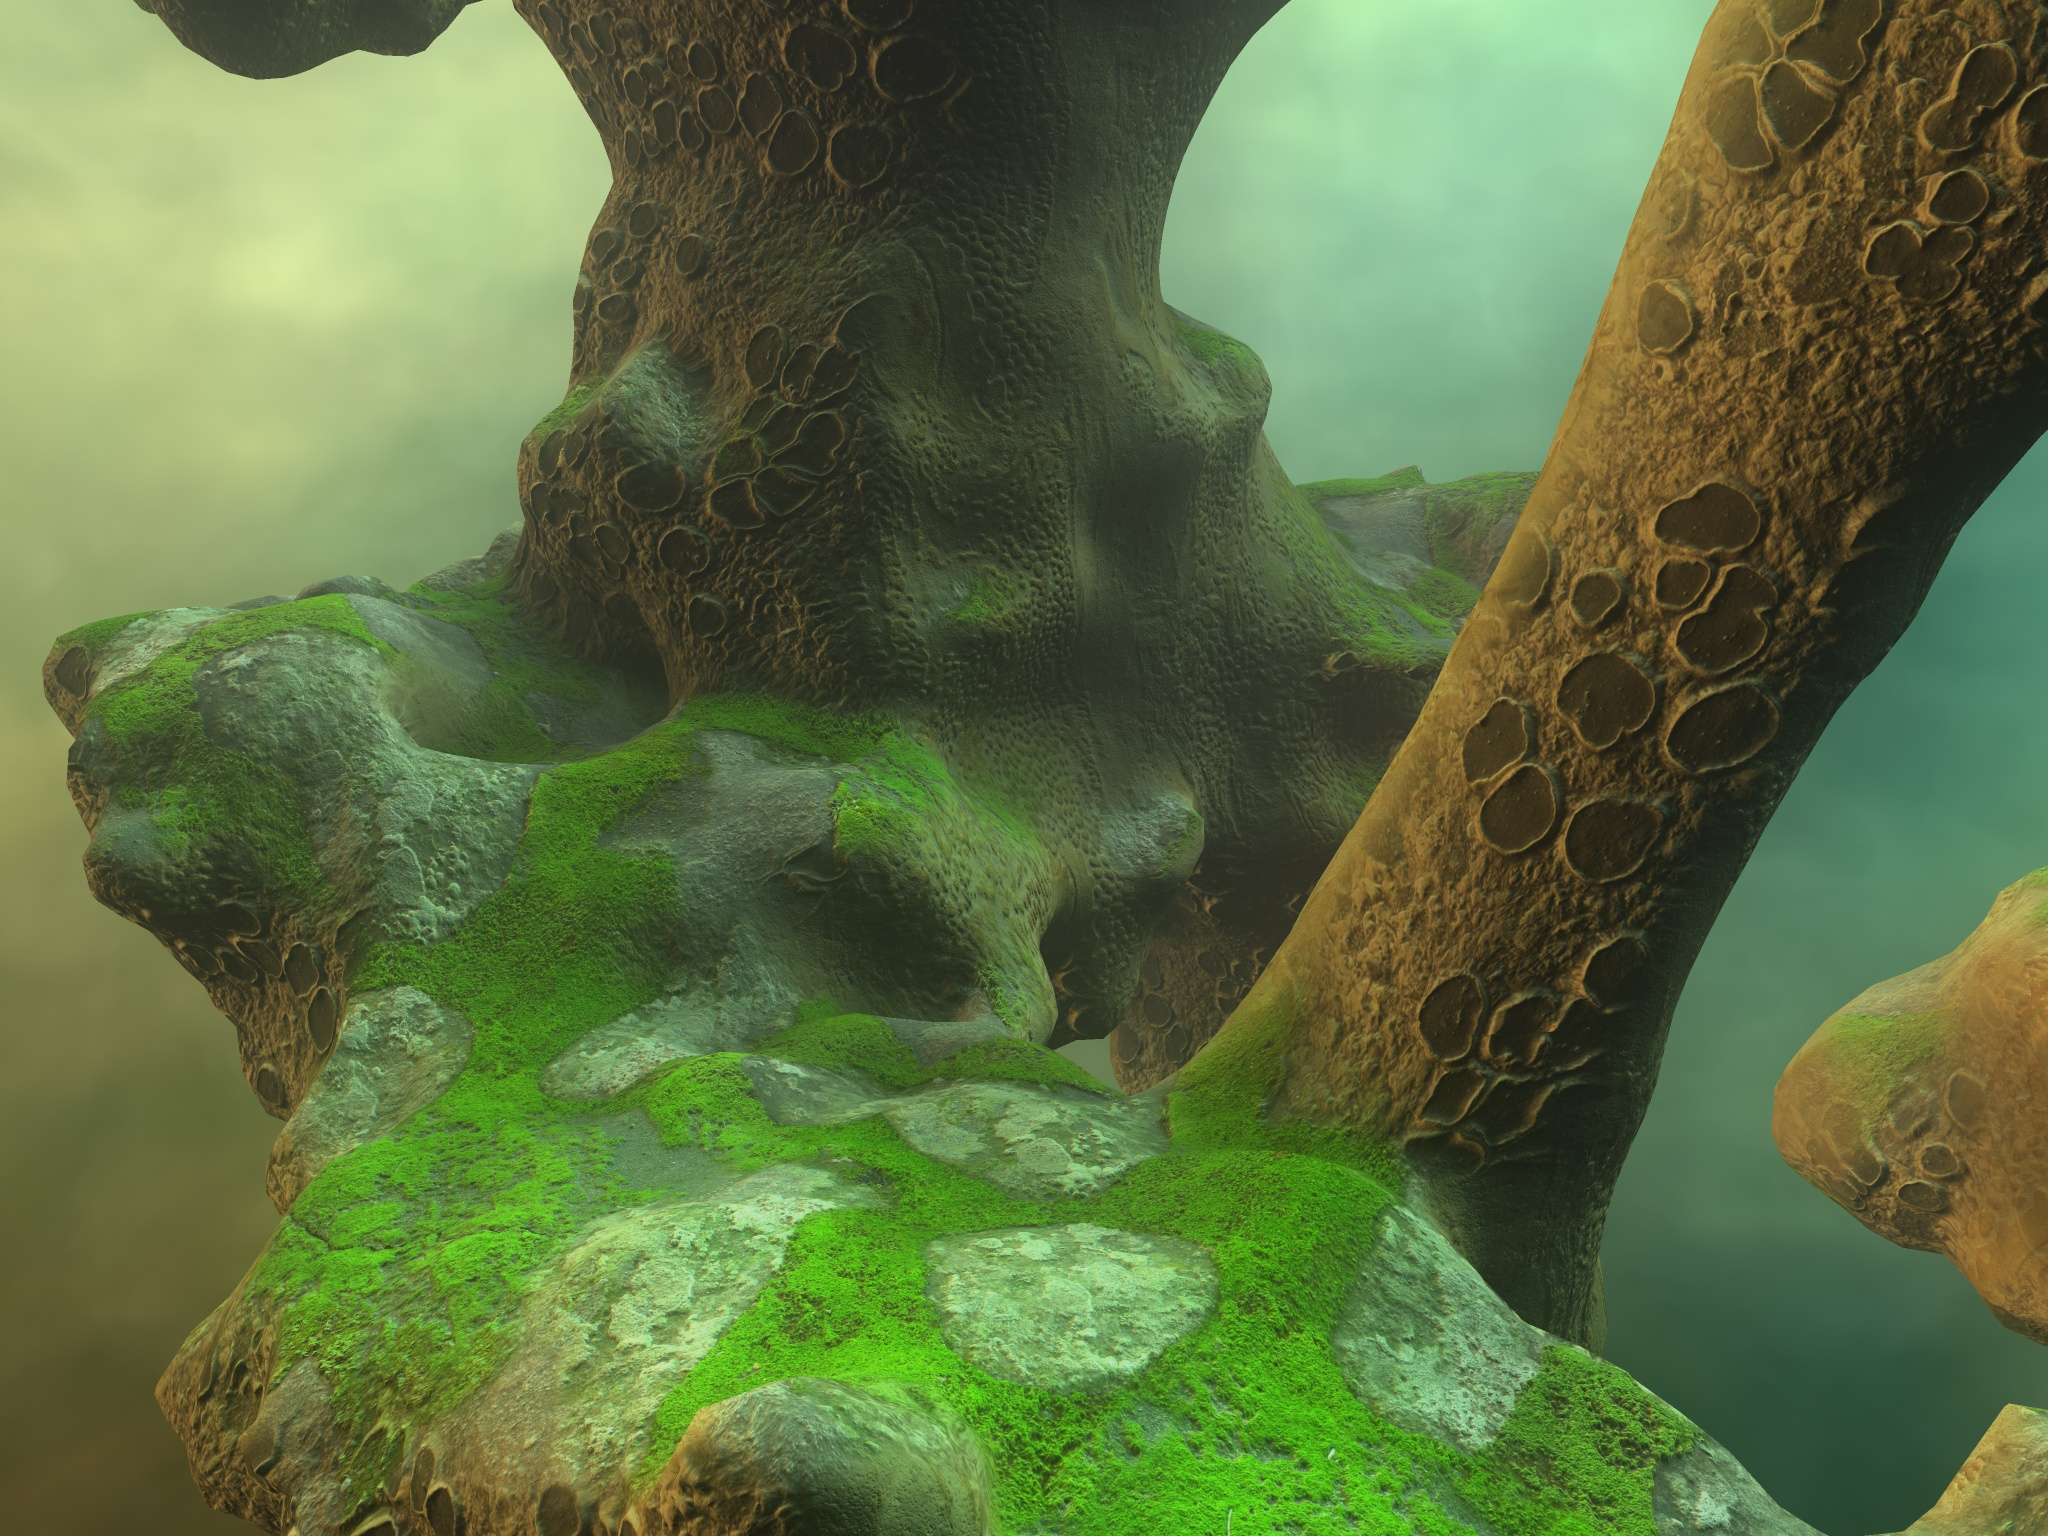
\includegraphics[width=0.5\linewidth]{PICs/cascades}
	\caption{Example of a procedural generated rock. \protect\cite{nvidia::cascades}}\label{cascadesFigure}
\end{figure}

\section{Game Mechanics}
Now it comes to the most important part in this chapter of PCG because of its leading part in PCGML as a game mechanic — the use of PCG as a game mechanic! Firstly, games which are using PCG as a game mechanic are presented and examples of possible PCG core mechanics are given afterwards.

\subsection{Current Games}
Many games are using procedural generated content in their game nowadays but not all of them are using PCG as a game mechanic. Some games which are using PCG as a game mechanic are described in the following sections.
\subsubsection{Galactic Arms Race}
Initially a research project which is a perfect example of PCG-based core mechanics in a game \cite{game::galacticArmsRace}. Galactic Arms Race is a multiplayer space shooter game in which the player need to complete tasks and missions to progress through the game \cite{game::galacticArmsRace}. To complete tasks and missions, players need to flight around in space and try to kill enemies with different weapons. Highlight of the game are the particle system weapons which are used to defeat enemies whereas weapons are completely generated by a PCG algorithm which uses evolutionary AI algorithms to evolve and generate new weapons \cite{pcg::galacticArmsRace}. The AI in Galactic Arms Race creates and evolves weapons based upon actions, strategies and weapons which are used the most by a player \cite{pcg::galacticArmsRace} \cite{pcg::galacticArmsRace::evolvingContent}. Besides, a player can just possess three weapons at a time whereby new evolved weapons are continuously spawned in space and dropped by enemies and consequently, players need to decide which weapons they want to use and thus feed the AI with information about their preferences \cite{pcg::galacticArmsRace::evolvingContent}. In this case, a player functions as the fitness function of the evolutionary algorithm used by the overall PCG system \cite{pcg::galacticArmsRace::evolvingContent}.\\
In short, the novel weapon system represents the core mechanic of Galactic Arms Race which is created with a combination of PCG algorithms and evolutionary AI algorithms.

\subsubsection{Inside a Star-Filled Sky}
Is an almost completely procedural generated game in which a player needs to progress through levels to reach one of the highest stages of progress in the highscore \cite{game::insideAStarFilledSky}. Players need to fight enemies, collect items, power-ups or weapons to defeat enemies and get over to the next level. Each level is generated and can represent the inside of an enemy, item or another entity in the game which gives the player an infinite choice of possibilities on how to play the game. Moreover, players can move in or out of the recursively nested levels and every item which is collected or enemy is killed changes the random seed for generating the next level \cite{pcg::endlessWeb}. Players can even move into their own character to increase their power and more than 165000 basic weapon combinations are explorable due to PCG \cite{game::insideAStarFilledSky}.\\
Summarized, the core mechanic of Inside a Star-Filled Sky is heavily PCG-based and about exploring and progressing through generated levels with the help of generated weapons and items.

\subsubsection{Endless Web}
Is an entirely PCG-based game and thus uses PCG as its core mechanic \cite{pcg::endlessWeb}. It is about fighting the nightmares in human dreams and rescue the trapped ones and thus releasing dreamers from their fears. Goal of the game is to rescue six dreamers by exploring the world and make decisions on exploring new areas in the world which affects the parameters of the rescue progress and also the generation of new world parts \cite{pcg::endlessWeb}. For example, if a player kills an enemy then depending on the configuration it strengthens or weakens an associated challenge and furthermore changes the world \cite{pcg::endlessWeb}.\\
Summarized, Endless Web's core mechanic is about manipulating the generative space where players influence the changes of the world generation with their chosen decisions on how they are playing the game \cite{pcg::endlessWeb}.

\subsubsection{Other Games}
Games like Black \& White, Diablo, Dwarf Fortress, Elite, Eve Online, Roque, Spelunky or Minecraft are other good examples which made use of PCG and related mechanics as an important part in their game.

\subsection{Possible Core Mechanics}
There are quite a few possibilities for what PCG can be used as mechanics in games. As seen, some core mechanics aim at weapon creation and progressing through generated space with the help of generated or altered "helper" mechanisms. Apart from that promising ideas are also other noteworthy ideas:
\begin{itemize}
	\item One exciting idea is about using PCG for multiplayer games as a multi-instance PCG system given by \cite{pcg::futureOfPcgInGames}. A game could use a central PCG system which is separated into different and unique systems for each player and every content generation would affect the PCG systems of other players \cite{pcg::futureOfPcgInGames}. In that case, influencing other players with your own PCG system to work towards a specific goal would be the core mechanic of the game. For example, it could be used in a collaborative multiplayer game where each content generation causes a new content generated in the other's player space, and they must find a way to communicate how to achieve a mutual objective \cite{pcg::futureOfPcgInGames}. 
	\item There is a lot of research done in the generation of quests as well. \cite{pcg::questGenerator} introduced research on quests which are generated upon analysis of four existing \ac{MMORPG} and their quests. One could create a simulation game where players need to create random quests by doing interaction with the PCG system in order to provide an AI agent with missions which needs to be fulfilled to solve some other problems in the game and thus progress throughout the game.
	\item Another idea is to adapt existing and successful introduced game mechanics with a PCG-backend. For example, one could create a game like Tetris where the core mechanics of rotating a block generates new blocks. For example, every time the player rotates the block, the next block will be altered with evolutionary algorithms and changes their shapes to increase the difficulty. Moreover, the system could adapt its difficulty to the player's skills regarding the success or failure rate of using the new blocks to maintain an acceptable experience.
\end{itemize} 

%
% ------------------------------- NEW CHAPTER ------------------------------- %
%
\clearpage
\chapter{\acl{ML}}
\ac{ML} is such a huge topic so that it would go beyond the scope of this thesis if every type, approach, method and model of it would be explained in detail. Therefore, the next sections will describe important subjects of ML which can be useful to explain for the further use in PCGML. \\
But let us ask a question first: What is the difference between ML and AI and what is ML about actually? The fact is, there is no difference between ML and AI. In particular, ML developed from fields of research in AI and is thus a subset of AI. It concentrates on using mechanisms to learn from given data where data can be seen as experience for a given problem. For instance, a famous example of machine learning is an application where the machine can distinguish between apples and pears with the help of a given dataset of features for both apples and pears \cite{ai::book}. 

\section{Types}
Machine learning can be divided into 3 main types which all address a different kind of problem to solve and goal to achieve. You can classify types of supervised learning, unsupervised learning and reinforcement learning \cite{ml::book::developer}. Each of them is dedicated to a specific task where it fits best and creates the desired results.

\subsection{Supervised Learning}
This type of learning is a task driven approach of ML and is mainly used for predicting or rather approximating data based upon existing historical or empirical values where the answer to the problem is already known \cite{ml::book::developer} \cite{ai::book}. The previous described problem of classifying apples and pears is a problem which is solved via supervised learning by predicting the specific class or fruit \cite{ml::book::developer}. In this case, we would provide a sample set of real data with features for both fruits and classify each feature to a specific fruit. With this, the algorithm links the given features to a specific result and is able to predict those fruits based upon a given test set \cite{ml::book::developer}. A training and test set could exist out of a bunch of pictures or other specific features described with numeric values in a table for each fruit. Hence, the reason why this is called supervised learning is due to the fact that the ML algorithm is provided with data and therefore knows what to learn \cite{ai::book}.\\
Common applications for supervised learning are for example, image recognition and classification, spam detection, pattern detection, speech recognition, \ac{NLP}, sentiment analysis or forecasting \cite{ml::book::algorithms}.

\subsubsection{Regression}
This technique of supervised learning is based on a statistical process where predictions are made on some particular probability distributions of the given training data \cite{ml::book::developer}. In specific, a regression algorithm is processing independent and dependent variables of a given problem and build relationships between them which are furthermore used to predict the correct answers of a given unknown set \cite{ml::book::developer}. Independent variables are describing features and dependent variable the meaning or outcome of a regression problem. Usually, regression algorithms are used when the output values are continuous prediction problems like for example, the predicted time of completion for a game level \cite{ai::book}.\\
The concept of regression algorithms could be used, e.g. for imitation and prediction of a player's behavior or player preference learning \cite{ai::book}. Some popular used algorithm for regression are linear or polynomial regression, \ac{ANN} or \ac{SVM}. \cite{ai::book}

\subsubsection{Classification}
Addresses problems where classification transition of independent values into specific values is needed \cite{ai::book}. The popular problem of classifying and distinguish apples and pears from each other falls into this section.\\
Like regression algorithms, classification algorithms could be used for imitation and prediction of a player's behavior, such as prediction of completion time \cite{ai::book}. But in this case, the possible output are specific values or classes like slow, average or fast instead of continuous values \cite{ai::book}. Some popular used algorithm for classification are, e.g. \ac{ANN}, decision tree, random forests, \ac{SVM}, K-nearest neighbor or ensemble learning \cite{ai::book}.

\subsection{Unsupervised Learning}
In contrast to supervised learning, unsupervised learning is based upon a data driven approach where the algorithm has no information about the meaning or value of any sample and needs to infer it automatically \cite{ml::book::developer}. Hence, an unsupervised learning algorithm gets so called unlabeled data without having a specific relationship to the target output and finds unknown structures and pattern in that set \cite{ai::book}. Going back to the apples and pears example, an algorithm would try to detect that there are 2 different types or classes in the dataset instead of predicting if its an apple or a pear.\\
Unsupervised learning is often used for object segmentation, similarity and pattern detection, automatic labeling, to pre-train supervised algorithms or pre-process data such as data compression, noise smoothing or outlier detection  \cite{ml::book::algorithms} \cite{ai::book}.

\subsubsection{Clustering}
For example, solves the previous described apples and pears problem by clustering apples and pears out of a given training set with features of both fruits. Based upon the learned knowledge of the training set, it is able to differentiate new and unknown samples into either apples, pears or a completely new class \cite{ai::book}. In detail, clustering algorithms are looking for similarities between given features and values and by doing this, they are inferring a relationship between them and thus separate specific classes \cite{ml::book::developer}.\\
Popular used algorithms for clustering are, e.g. K-Means, neural networks or hidden markov models. \cite{ml::book::developer}

\subsection{\acl{RL}}
In short, \ac{RL} is an goal-oriented approach which uses so called agents who are used to get feedback or specific states of an environment which is further used to learn and improve new decisions based on taken decisions \cite{ml::book::developer}. Inspired by the way humans and animals learn to take decisions, it aims at rewarding the algorithm for good behavior and thus leads it towards the best knowledge and output \cite{ai::book}. \\
In detail, there is a bit of supervision used in form of feedback for an action executed by an agent which is usually referred as the reward for an action \cite{ml::book::statistics}. Tricky part is, that RL consists of sequential decisions and every chosen action, which can be chosen out of a set of actions, by an agent is changing the environment which usually makes it difficult to train a model \cite{ml::book::statistics}. Hence, an agent executes different decisions in a loop and is looking for the highest total reward for its sequence of actions since it will always want to increase his total reward. \cite{ai::book} With this strategy, an RL algorithm is getting better and better over time in solving a specific problem until it found the best solution.\\
During the last years, RL algorithms have been used to learn an AI how to play classical games, find the best strategy to win a game, learn an AI how to walk and many other applications \cite{ml::book::algorithms}. Algorithms include neural networks, deep neural networks, Q-Learning or markov decision process. \cite{ml::book::statistics}

\begin{comment} it doesn't make any sense to describe all learning models for machine learning if they won't be used at all?!
\section{Learning Models}
Which training models are used in ML? --> the 5 tribes of ML\\
"A Machine Learning model is a set of assumptions about the underlying nature the data to be trained for. The model is used as the basis for determining what a Machine Learning algorithm should learn. A good model, which makes accurate assumptions about the data, is necessary for the machine to give good results" \cite{ml:3}\\
each model has its pros and cons and therefore it is not useful to compare each of them without a specific problem or game mechanic problem which should be solved. furthermore, a short description about it as well as pros and cons of their usages shall be given to introduce them. (NO CITE)

\subsection{Linear}
used for regression \cite{ml:2}

\subsection{K-Nearest Neighbor}
used for classification \cite{ml:2}\\
\cite{ml::book::developer} page 72 - 80\\
\cite{ml::book::statistics} page 187 - 202

\subsection{Decision Tree}
\cite{ml::book::algorithms} page >154\\
used for classification \cite{ml:2}\\
\cite{ml::book::statistics} page 119\\
supervised, can be used for either classification, prediction or preference learning tasks. \cite{ai::book}\\
In decision tree learning [67], the function f we attempt to derive uses a decision tree representation which maps attributes of data observations to their target values. The former (inputs) are represented as the nodes and the latter (outputs) are represented as the leaves of the tree. The possible values of each node (input) are represented by the various branches of that node. The goal of decision tree learning is to construct a mapping (a tree model) that predicts the value of target outputs based on a number of input attributes.\cite{ai::book}

\subsection{\acl{SVM}}
\cite{ml::book::algorithms} page >133\\
used for classification \cite{ml:2}\\
\cite{ml::book::statistics} page 214 - 240\\
supervised; alternative and very popular set of supervised learning algorithms that can be used for either classification, prediction or preference learning tasks. is a binary linear classifier that is trained so as to maximize the margin between the training examples of the separate classes in the data (e.g., apples and pears). SVMs have been used widely for text categorization, speech recognition, image classification, and hand-written character recognition among many other areas.\cite{ai::book}\\
Similarly to ANNs, SVMs construct a hyperplane that divides the input space and represents the function f that maps between the input and the target outputs. Instead of implicitly attempting to minimize the difference between the model's actual output and the target output following the gradient of the error (as backpropagation does), SVMs construct a hyperplane that maintains the largest distance to the nearest training-data point of any other class. That distance is called a maximum-margin and its corresponding hyperplane divides the points (xi) of class with label (yi) 1 from those with label -1 in a dataset of n samples in total. \cite{ai::book}\\
They are efficient in finding solutions when dealing with large, yet sparse, datasets as they only depend on support vectors to construct hyperplanes. They also handle well large feature spaces as the learning task complexity does not depend on the dimensionality of the feature space. SVMs feature a simple convex optimization problem which can be guaranteed to converge to a single global solution. Finally, overfitting can be controlled easily through the soft margin classification approach. \cite{ai::book}

\subsection{Neural Networks}
used for regression \cite{ml:2}\\
\cite{ml::book::developer} page >131

\subsubsection{\acl{ANN}}
\cite{ml::book::algorithms} page 289\\
\cite{ml::book::statistics} page 241 - 267\\
supervised, can be used for either classification, prediction or preference learning tasks. but also unsupervised \cite{ai::book}\\
Artificial Neural Networks (ANNs) are a bio-inspired approach for computational intelligence and machine learning. An ANN is a set of interconnected processing units (named neurons) which was originally designed to model the way a biological brain—containing over $10^{11}$ neurons—processes information, operates, learns and performs in several tasks. Biological neurons have a cell body, a number of dendrites which bring information into the neuron and an axon which transmits electrochemical information outside the neuron. The artificial neuron (see Fig. 2.12) resembles the biological neuron as it has a number of inputs x (corresponding to the neuron dendrites) each with an associated weight parameter w (corresponding to the synaptic strength). It also has a processing unit that combines inputs with their corresponding weights via an inner product (weighted sum) and adds a bias (or threshold) weight b to the weighted sum as follows: $x*w+b$. This value is then fed to an activation function g (cell body) that yields the output of the neuron (corresponding to an axon terminal). ANNs are essentially simple mathematical models defining a function $f : x \rightarrow y$. \cite{ai::book}\\
core applications: pattern recogintion, robot and agent control, game-playing, decision making, gesture, speech and text recognition, medical and financial applications, affective modeling, and image recognition \cite{ai::book}\\
pro: compared to other supervised learning approaches is their capacity to approximate any continuous real-valued function given sufficiently large ANN architectures and computational resources. This capacity characterizes ANNs as universal approximators \cite{ai::book}\\
\subsubsection{\acl{CNN}}
\cite{ml::book::developer} page >158
\end{comment}

\section{Development}
How to use PCG and ML in a game engine? What are some of the best practices and approaches for using PCG and ML in a game?

\subsection{Design Considerations}
"AI must be robust enough to support player experimentation and exploration, and games must be designed to take full advantage of it." \cite{ai::gameDesign}\\
"Systems that are completely predictable to the player feel mechanical and “dead”" \cite{ai::gameDesign}\\
"we cannot merely write a new AI system and expect that this alone will create a new experience." \cite{ai::gameDesign}\\
When discussing AI-based game design, it is useful to use the Mechanics, Dynamics, and Aesthetics (MDA) framework \cite{ai::gameDesign}\\
An AI-based game is one that has an AI system closely integrated into its core mechanics and aesthetics, and also into the setting and story. \cite{ai::gameDesign}\\
At the core of the AI-based game design process is this iterative loop involving the AI design and game design informing each other in an iterative manner. \cite{ai::gameDesign}\\
Without a rough design of the AI system, it is impossible to flesh out the mechanics of the game; without a rough design of the game system, it is impossible to know what should be modeled in the AI system. \cite{ai::gameDesign}\\
The game and AI designs are each also informed by the domain of the project. There are typically at least three types of domains used during AI-based game design: AI architectures, game design conventions, and knowledge domains. \cite{ai::gameDesign}\\
\\
we have distilled two major discussion points: the importance of maintaining an appropriate level of transparency of the AI system through the game design, and the challenges of designing for emergent gameplay.\cite{ai::gameDesign}\\
transparency of the AI-system: However, from a gameplay perspective, it is also important not to overwhelm the player with too much information about the AI system. Finding the appropriate level of transparency for the AI system, or the amount of the AI system that is exposed to the player, is a delicate balancing act.\cite{ai::gameDesign}\\
emergent gameplay: Emergent gameplay is a fundamental quality of an AI-based game, as the player is supported by an underlying system that can respond intelligently to the player’s actions. For emergence to occur, it is not necessary for the AI system itself to exhibit emergent behavior. For example, consider the following hypothetical game that is supported by an AI-system for pathfinding. The player must direct autonomous agents towards particular goals by manipulating terrain and forcing the agents to take a particular path. The AI system could always find only the optimal path for the lemmings, but its intelligent and rapid response to the player ensures a variety of strategies that the player can employ. \cite{ai::gameDesign}\\
machine learning can be frighten and if a player has interaction with the system, it should be as easy as possible so the player is not overwhelmed by the system and its possibilites! (MY WORDS)\\
\\
AI algorithm design: \cite{ai::book}
\begin{itemize}
	\item Representation of Game State: Depending on the AI system it is crucial that game states are described in a way so that the system can easily e.g. read and observe it.
\end{itemize}

supervised learning: Learning = Maximize Utility -> error function represents how well an approach maps training examples to target (desired) outputs \cite{ai::book}\\
unsupervised learning: Learning = Maximize Utility -> is often provided internally and within the representation via e.g., competitive learning or self-organization \cite{ai::book}\\
reinforcement learning: Learning = Maximize Utility -> reward, which is a function an agent attempts to maximize by learning to take the right action in a particular state. \cite{ai::book}\\

\subsection{Common Pitfalls}
Following pitfalls are commonly occurring problems when implementing and training machine learning models for a specific problem.

\subsubsection{Under- and Overfitting}
ML models are used to approximate unknown output based on given training data \cite{ml::book::algorithms}. When talking about fitting, then it is referred to fit a model to a given training set which is used to train the model. This set can consist of many independent variables and different entries which are applied to a model.
\begin{itemize}
	\item \textbf{Underfitting}: Happens when you train your model with too less information or independent variables so that your model is not able to capture the dynamics between the values \cite{ml::book::algorithms}.
	\item \textbf{Overfitting}: Is exactly the opposite of underfitting. When a model is over fitted then it is fed with too much information and variables so that it is not able to generalize the dynamic relationship of variables during the training \cite{ml::book::algorithms}.
\end{itemize}
So keep in mind to provide a good amount of information for the training of a machine learning model to achieve a good fitted model. A method to check and prevent your model from being over or under fitted is the technique of validation such as cross-validation which helps to detect those problems \cite{ml::book::algorithms}.

\subsubsection{Curse of Dimensionality}
This problem often occurs when the training set is smaller than the amount of feature variables, or also called the dimensions of a set, which are used to train a model \cite{ml::book::algorithms}. In this case, if the number of features increases then the performance of the model gets dramatically reduced \cite{ml::book::algorithms}. Possible ways to prevent and solve this problem are, e.g. a decrease of dimensions or providing more training data \cite{ml::book::algorithms}.

\subsection{Game Engine Plugins}
Basic sample PCG and ML implementations in a game engine.
\subsubsection{Unity}
\url{https://github.com/Unity-Technologies/ml-agents}
\subsubsection{Unreal Engine 4}
\url{https://github.com/getnamo/tensorflow-ue4}

\section{Game Mechanics}
\subsection{Current Games}
there are a some AI-based games with AI-based game mechanics (Pataphysic Institute, Prom Week, Mismanor, Endless Web, MKULTRA, A Rogue Dream) \cite{ai::aiBasedGameDesignPattern}\\
\\
The most common application of machine learning is to optimize the policy that controls non-player characters (NPCs). For example, the ANN race car controllers Colin McRae Rally 2.0 and Forza Motorsport 2 and the creature brains in Creatures 3 and Black and White 2 are learned. \protect\cite{pcg::galacticArmsRace::evolvingContent}\\
"As a real world example, induction on decision trees was used in Black and White, as the creature learnt to predict the player's reaction. Every time the creature did something, it recorded the player's reaction (slap, reward, etc.), and used this action-player feedback tuple as the input to an induction mechanism to build the decision tree that conditions future action selection. This way the creature ended up doing the kind of actions the player rewarded, and avoided the rest." \url{https://www.gamasutra.com/view/feature/130633/postcard_from_gdc_2005_tutorial__.php}
\subsection{Possible Mechanics}
\cite{ai::aiBasedGameDesignPattern} introduced nine design patterns which illustrates ways to develop game mechanics based on AI techniques and furthermore to create AI-based games. (should probably read every part again when writing this chapter)

\subsubsection{AI as Visualized}
Pattern: Provide a visual representation of the underlying AI state, making gameplay revolve around explicit manipulation of the AI state.\\
What player(s) do: Observe AI state\\
Role of AI (in relation to player): Gives (strategic) information, showing states
\subsubsection{AI as Role-Model}
Pattern: Provide one or more AI agents for the player to behave similarly to.\\
What player(s) do: Imitate AI\\
Role of AI (in relation to player): Show agent actionas and behaviors, agents as puzzles
\subsubsection{AI as Trainee}
Pattern: Have player actions train an AI agent to perform tasks central to gameplay. \\
What player(s) do: Teach AI\\
Role of AI (in relation to player): Child/student\\
Explanation: Machine learning techniques revolve around learning new behaviors using examples. By using player actions as a source of examples an AI agent can learn to perform tasks, with this indirect control (or automation) becoming central to player activity in a game. Note that many paradigms for training exist. Supervised learning requires players to explicitly provide feedback by labeling examples as indicative of a behavior. Unsupervised learning abstracts from examples without explicit guidance. Reinforcement learning uses feedback about the value of actions, rather than labels describing what an action was. Each of these paradigms provides opportunities for different kinds of player action in a game to indirectly control game outcomes.
\subsubsection{AI as Editable}
Pattern: Have the player directly change elements of an AI agent that is central to gameplay.\\
What player(s) do: Edit AI\\
Role of AI (in relation to player): Artifact/agent that player can author/manipulate
Game: Galactic Arms Race
\subsubsection{AI as Guided}
Pattern: The player assists a simple or brittle AI agent that is threatened with self-destruction.\\
What player(s) do: Guide/manage the AI\\
Role of AI (in relation to player): Partly independent inhabitants, with players as their Gods
\subsubsection{AI as Co-Creator}
Pattern: Involve the player in a creative task where an AI agent directly contributes to the task as an equal partner.\\
What player(s) do: Make artifacts assisted by AI\\
Role of AI (in relation to player): Co-creator, making artifacts
\subsubsection{AI as Adversary}
Pattern: Require players to overcome an (embodied or not) AI opponent in a contest.\\
What player(s) do: Play game against the opponent\\
Role of AI (in relation to player): Opponent (symmetric)
\subsubsection{AI as Villain}
Pattern: Require players to complete a task or overcome an AI opponent where the AI is aiming to create an experience (e.g., tension or excitement) rather than defeat the player.\\
What player(s) do: Combat the Villain(s)\\
Role of AI (in relation to player): Villain in game; mob, boss mob, NPC (asymmetric)
\subsubsection{AI as Spectacle}
Pattern: Have an AI or group of AI agents implement a complex system, such as a social hierarchy, that the player may observe or interfere with.\\
What player(s) do: Observe\\
Role of AI (in relation to player): Spectacle, enacting simulated society


%
% ------------------------------- NEW CHAPTER ------------------------------- %
%
\clearpage
\chapter{\acl{PCGML}}
\cite{ai::book} p 173-175
\section{What is it About?}
Theory of PCGML and its methods in general.
Evaluation of PCGML hardware and software requirements
\section{Current Use in Games}
\section{Possibilities}
\section{Difference to Usual \acl{PCG}}
The core difference between PCG via machine learning and approaches such as search-based PCG is that the content is created directly (e.g., via sampling) from models which have been trained on game content. \cite{ai::book}
\section{Example Implementations}
Theory of PCGML and its methods in general.
\section{Learning Models}
Comparison of PCGML learning models
\subsection{Markov Chains}
\subsection{\acl{ANN}}
\cite{ml::book::algorithms} page 289
\subsection{Bayes}
\cite{ml::book::algorithms} naive bayes: page >120\\
\cite{ml::book::statistics} naive bayes: page 203 - 219\\
look for a paper of "Guzdial"
\section{In a Game Engine}
research on different PCGML implementations and practical usage possibilities in a game engine
\subsection{Conceptual Prototype}
\subsection{Possible Issues}
%
% ------------------------------- NEW CHAPTER ------------------------------- %
%
\clearpage
\chapter{\acl{PCGML} Game Mechanics}
the design process for \cite{pcg::endlessWeb} followed the principles of \cite{ai::gameDesign} with Launchpad as the AI system.

\section{First Considerations}

\section{Concepts of Possible Mechanics}
maybe read over \cite{pcg::endlessWeb} again\\
read explanation of design pattern in \cite{ai::aiBasedGameDesignPattern} again!

\subsection{Role-Model}
"A \ac{PCGML} system replicates content which is generated by players of various levels of skill or generates content suitable for players of certain skill levels. New players are trained by replicating the content or by playing the generated content in the form of generative tutorial." \cite{pcgml::paper}

\subsection{Trainee}
"The player trains a \ac{PCGML} system to generate a piece of necessary content (e.g., part of a puzzle or level geometry)." \cite{pcgml::paper}

\subsection{Editable}
"Rather than training the AI to generate the missing puzzle piece via examples, the player changes the internal model’s values until acceptable content is generated." \cite{pcgml::paper}

\subsection{Guided}
"The player corrects the \ac{PCG} system’s output to fulfil increasingly difficult requirements. The \ac{AI}, in turn, learns from the player’s corrections, following the player’s guidance." \cite{pcgml::paper}

\subsection{Co-Creator}
"The player and a \ac{PCGML} system take turns in creating content, moving towards some external requirements. The \ac{PCGML} system learns from the player’s examples." \cite{pcgml::paper} 

\subsection{Adversary}
"The player produces content that the \ac{PCGML} system must replicate by generation to survive or vice versa in a “call and response” battle." \cite{pcgml::paper}

\subsection{Spectacle}
"The \ac{PCGML} system is trained to replicate patterns that are sensorically impressive or cognitively interesting." \cite{pcgml::paper}

\section{Conceptual Prototypes (with evaluation)}
A test implementation of PCGML game mechanics in a game engine.

\subsection{Comparison of Different Mechanics}
Comparison of implemented PCGML game mechanics prototypes.

\section{Summary}
what is the best game mechanic? why? etc
%
% ------------------------------- NEW CHAPTER ------------------------------- %
%
\clearpage
\chapter{Game Prototype}
Development of a game with one of the best-evaluated PCGML game mechanic as the central game mechanic of the game.
\section{Considerations}

\subsection{Which Game Engine?}
There are 2 main engines which are commonly used thorough the industry due to their fact of free to use.

\section{Game Design}
\textbf{Designing Awesome AI for Games - Summary (GDC Talk)}
\begin{enumerate}
	\item Support the core experience
	\item Watch people play and get in their heads
	\item Identify broad behaviours
	\item Start simple
	\item Figure out what the brain gives you for free
	\item Try going simpler before you go complex
\end{enumerate}

\section{Implementation}
\subsection{Technical Approach}
Classes, Diagrams, why use what - eg. why use neural network over other and stuff like that!
\subsection{Online or Offline?}
\section{Performance Measurements}
\subsection{Improvement Iterations}
\section{Playtest}
\subsection{Preparations}
\subsection{Evaluation}
Evaluation of playtesters feedback.
\section{Result}
show the game and the mechanics!

%
% ------------------------------- NEW CHAPTER ------------------------------- %
%
\clearpage
\chapter{Conclusion}
The meaning of the use of PCGML as a game mechanic for the future of games and gaming. 
\section{Summary}
\section{Research Result}
\section{Future Work}
%
% Hier beginnen die Verzeichnisse.
%
\clearpage
\ifthenelse{\equal{\FHTWCitationType}{HARVARD}}{}{\bibliographystyle{gerabbrv}}
\bibliography{Literatur}
\clearpage

% Das Abbildungsverzeichnis
\listoffigures
\clearpage

% Das Tabellenverzeichnis
\listoftables
\clearpage

% Das Quellcodeverzeichnis
\listofcode
\clearpage

\phantomsection
\addcontentsline{toc}{chapter}{\listacroname}
\chapter*{\listacroname}
\begin{acronym}[XXXXX]
	\acro{2D}{2-Dimensional}
	\acro{3D}{3-Dimensional}
	\acro{AI}{Artificial Intelligence}
	\acro{ANN}{Artificial Neural Network}
	\acro{CNN}{Convolutional Neural Network}
	\acro{GB}{Gigabyte}
	\acro{MDA}{Mechanics-Dynamics-Aesthetics}
	\acro{ML}{Machine Learning}
	\acro{MMORPG}{Massively Multiplayer Online Roleplay Game}
	\acro{NLP}{Natural Language Processing}
	\acro{PC}{Personal Computer}
    \acro{PCG}{Procedural Content Generation}
    \acro{PCGML}{Procedural Content Generation via Machine Learning}
    %\acro{RPG}{Roleplay Game}
    \acro{RL}{Reinforcement Learning}
    \acro{RNG}{Random Number Generator}
    \acro{SVM}{Support Vector Machine}
\end{acronym}

%
% Hier beginnt der Anhang.
%
\clearpage
\appendix
%\chapter{Appendix A}
\end{document}